\documentclass{article}

% --- load packages ---

\usepackage[margin=1in]{geometry} % change the margins
\usepackage{amsmath} % useful math environments and commands like align
\usepackage[colorlinks,bookmarks,bookmarksnumbered,allcolors=blue]{hyperref} % hyperlinks between references
\usepackage{graphicx}  % include images
\usepackage[caption=false]{subfig} % subfigures.  false option prevents conflicts in caption styling with other packages
\usepackage{booktabs} % better tables
\usepackage[capitalise]{cleveref} % better referencing. uses cref.
\usepackage[section]{placeins} % sometimes useful to prevent figures from floating out of a section
\usepackage{cite} % handles multiple citations in one command better
\usepackage{doi} % allow correct hypderlinking of DOIs
\usepackage{hyperref}


\begin{document}

\title{Homework 3}
\author{Jaron Ellingson}
% put in \date{} if you don't want a date to appear, or enter a specific date, otherwise default is today's date.
\maketitle

 %\href{https://byu.box.com/shared/static/anxheci3eytucrh3ke57k2sqdx0ivmjg.pdf}{homework pdf}

\section*{Computing Derivatives}

The following describes and compares several methods for computing derivatives for constrained optimization problems. I choose to implement these methods to solve a 10 member truss problem which seeks to the mass of a 10-truss structure that holds a load suspended horizontally from a wall (\cref{fig:truss}). This problem 

\begin{equation*}
\begin{aligned}
\text{minimizes} & \quad J= \sum_{i=1}^{n} Mass(A_i) \\
\text{with respect to} & \quad A_1 ... A_{n} \\
\text{subject to} & \quad A_i \ge 0.1 \quad \text{and} \quad | \sigma_i | \le \sigma_y \quad \forall i=1 ... n,
\end{aligned}
\end{equation*}

where $A_i$ is the cross-sectional area, $\sigma_i$ is the corresponding stress, and $\sigma_y$ is the yield stress. Please see this see \href{https://byu.box.com/shared/static/h8gzy7nuzzk42ta7388y1luj3yhgsltq.pdf}{handout} for further details.


\begin{figure}[htbp]
	\centering
	
	\includegraphics[width=0.75\textwidth]{truss.png}
	
	\caption{Truss}
	\label{fig:truss}
\end{figure}

To effectively solve this problem, the optimization methods requires derivatives to be computed. More precisely we need the function  and constraint derivatives or 


\begin{equation}
\frac{\partial m}{\partial A}=
\begin{bmatrix} 
\frac{\partial m}{\partial A_1} \\
\vdots \\
\frac{\partial m}{\partial A_{n_x}}
\end{bmatrix}
\end{equation}

and 

\begin{equation}
\frac{\partial \sigma}{\partial A}=
\begin{bmatrix} 
\frac{\partial \sigma_1}{\partial A_1} & \dots & \frac{\partial \sigma_i}{\partial A_{n_x}} \\
\vdots & \ddots & \\
\frac{\partial \sigma_{n_f}}{\partial A_1} &        & \frac{\partial \sigma_{n_f}}{\partial A_{n_x}} 
\end{bmatrix},
\end{equation}

where m is the mass of the truss, $n_x$ is the number of truss areas, and $n_f$ is the number of constrained stress elements. In this problem $n_x=n_f$.

\subsection*{Finite Difference}

\subsection*{Complex Step}

\subsection*{Algorithmic Differentiation}

\subsection*{Adjoint}




\href{https://byu.box.com/shared/static/17bqmaop0v1o0fwqg1etx7dofl6ad35t.pdf}{textbook} 
\section*{Truss Derivatives}

\begin{table}[htb]
	\centering
	\caption{Average relative error for each method with 1000 uniformly random starting points.}
	\label{tab:comp_der}
	\begin{tabular}{c|c|c}
		\toprule
		Algorithm & Mass Derivative & Stress Derivative \\
		\midrule
		Finite-Difference & 5.347291203789755e-05 & 0.02727215090088324 \\
		Complex-Step  & 0.0 & 3.336212472827231e-10 \\
		Algorithmic Differentiation & 0.0 & 2.1207032039874913e-11 \\
		\bottomrule
	\end{tabular}
\end{table}

\section*{Truss Optimization}

\begin{table}[htb]
	\centering
	\caption{a.}
	\label{tab:c}
	\begin{tabular}{c|c|c}
		\toprule
		Algorithm & Function Evaluations & Time (sec) \\
		\midrule
		Finite-Difference & 386.0 & 3.3085175704956056\\
		Adjoint & 32.96 & 0.25411544799804686 \\
		\bottomrule
	\end{tabular}
\end{table}

\begin{figure}[htbp]
	\centering

	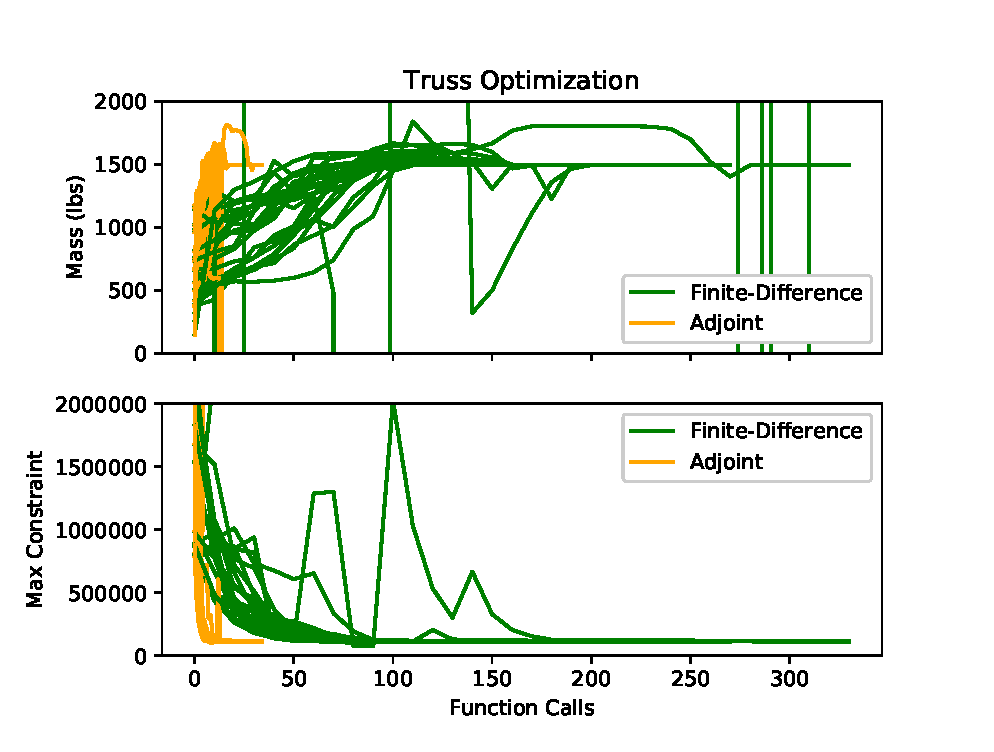
\includegraphics[width=0.75\textwidth]{optimality10.eps}

	\caption{optimality10}
	\label{fig:opt10}
\end{figure}



% This is for the bibliography.  Note that it is using sample.bib 
% you would need to provide your own bibtex file.

\bibliographystyle{unsrt}
\bibliography{sample}




\end{document}